% intro
Machine learning (ML) have many applications in experimental particle physics, such as event identification and reconstruction which include calorimeter cluster calibration, which is the focus of this thesis. This chapter introduces some background on the used ML methods which covered in the next chapters. %(Check this source for more info and source).

Before talking about ML, we need to introduce Artificial intelligence (AI). AI is the process of computers being trained to imitate how the human brain learns and solves problems. An AI computer program, software, could be simple as a chess game or complex as one that can predict the RNA structure of a virus to help develop vaccinee %source1.  
There are different types of AI, as shown in the related figure, and ML is a subsection of AI and deep learning (DL) is a subsection of ML. To understand the difference between ML and DL, ML is of AI where it needs a human intervene to improve its learning and DL where computers learn from its own past mistakes. %(Source for more info about deep learning.)

In ML there are few concepts to be familiar with, such as Al algorithm, and ML model. (fix me- these concepts will be used a lot in the next chapters). An AI algorithm is a set of instructions, programming, that tells the computer how to learn to operate on its own (%source2) 
to solve a problem or do a task. ML models are computer programs used to recognize patterns in data (classification) or make predictions (regression). ML models are created using ML algorithms that undergo a training process with a data to modified the algorithm to be better at manage the specific task and becomes a ML model. % Source3

ML algorithms could be categorized into three main groups depending on type of data used in the training process: supervised learning, unsupervised learning, reinforcement learning, as seen in figure related. (% source) 
Data could be labeled, unlabeled. Labeled data is any data the has an attribute or category assigned to for example like the price of a product or the height of a human. For ML algorithms and model implementation various python-based libraries, such as schitkit-learn, TensorFlow, and keras are used. In this chapter will describe the most commonly used ML algorithms in HEP %source 
: boosted Decision trees and Neural networks.


\begin{figure}[t!]
\centering
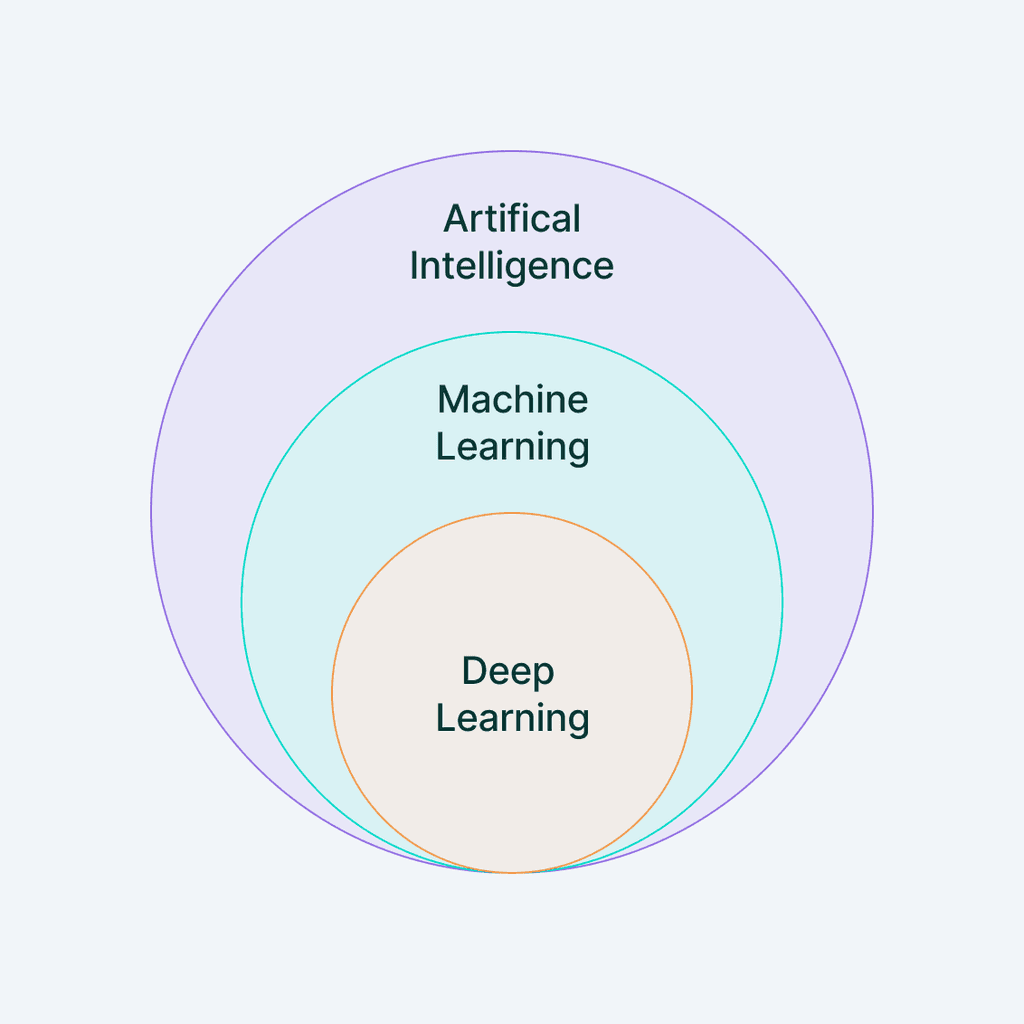
\includegraphics[width=0.99\textwidth]{figures/ML_diagram.png}
\caption[ML and AI]{}. Figure source~\cite{SMtable}.
\label{fig:ML_diagram}}                                                                                                                                                                                        
\end{figure}
  
\section{BDT}
A decision trees (DT) ,as seen in the related figure, is a type of algorithm that looks like an upside-down tree that starts with a root at the top, and then branches out to leaves. A DT has different level of nodes: Root node is top most node and it represent the entire message of the decision. Decision node is a node where the prior node branches into two or more. Leaf node is the last node in DT and there furthers from the root node. DTs are supervised learning algorithms that can be used to make classification and regression models (this thesis deal with regression problems).

In DT each node the split is chosen to maximalize the information gain (difference between in entropy before and after the potential split), in other words minimizing the entropy. Entropy is max for 50/50 split and mini for 1/0 split. The spilt is created reclusively (iteratively) and this process is repeated until some stop condition is met, ex: depth of tree no more information gains etc.

In boosted decision trees (BDT), DT uses a boosting technique that iteratively works to improve the weak trees by combining more, tree, that will correct the error of the previous one. How this works, the new tree will be trained on the samples that were misclassified by the previous tree which gradually will refine the overall accuracy (fix me).  In BDT, the final prediction is the weighted average of all models (trees) with more weight given to those with higher accuracy.  There are different ways to iteratively adding learners %to minimize a loss function 
most common ones for example are Adaboost (adaptive boosting), Gradient boosting, XGBoost which will be used later for ECAL CAL.

\section{NN}
Neural Networks (NN), also called artificial neural (ANN) networks because of how they mimic the neurons in the brain sending signals to each other. 
They are one of the most used ML algorithms (in particle physics). 
The simplest NN contains an input layer, output layer, and one hidden layer each containing number of neurons that are connected. NN’s are the backbone of DL algorithms if they have more one hidden layer. %(insert picture of a simple NN vs DL with multiple layers)

NN like other DL algorithms relay on the training data to learn to improve its accuracy overtime without human intervention. As mentioned before each layer have multiple neurons and each one of those neurons (could think of it as its one linear regression model, activation function) contains input data, weights, bias, and output. (fix me)

All inputs then multiplied by their respective weights (helps determine the importance of any given variable) and then summed. Afterward the output (with bias) is passed through the activation function (example of activation function?) if the output exceeds a given threshold, it activates the node and passing data to the next layer in the network. This results in the output of one node becoming in the input of the next node. This process of passing data from one layer to the next layer defines this NN as feedback network. The goal is minimizing errors (cost/loss function, example) to insure the fitting of the model. As the model adjusts its weight and bias. Until reaches a local minimum (mention gradient decent).










